\documentclass[12pt,a4paper]{article}

\usepackage[utf8]{inputenc}
\usepackage[T2A]{fontenc}
\usepackage[ukrainian]{babel}

\usepackage{geometry}
\geometry{left=2cm,right=2cm,top=2cm,bottom=2cm}

\usepackage{graphicx}
\usepackage{array,multirow}
\usepackage{booktabs}
\usepackage{caption}
\renewcommand{\thetable}{\arabic{table}}
\captionsetup[table]{name=Таблиця}

\usepackage{amsmath}
\usepackage{pdflscape}
\usepackage{xcolor}

\usepackage{hyperref}

\begin{document}

    \begin{titlepage}

        % Картинка шапки (по центру, з відступом від верху)
        \begin{center}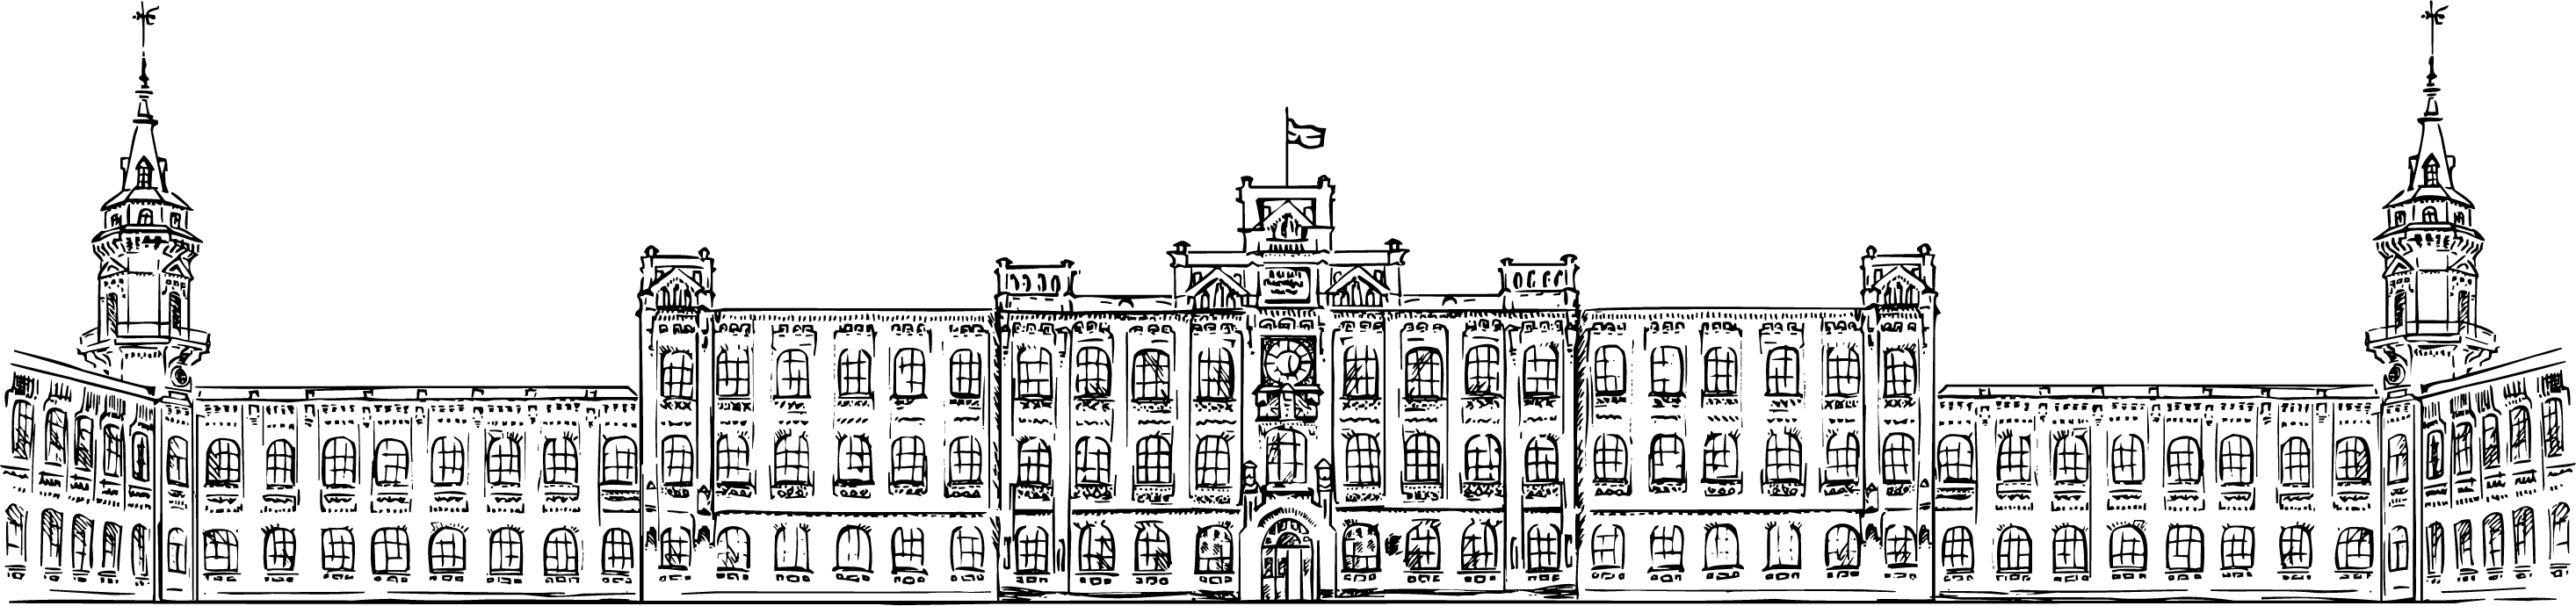
\includegraphics[width=0.7\textwidth]{letterhead.png}\end{center}

        \begin{center}
            \large Національний технічний університет України\\
            «Київський політехнічний інститут імені Ігоря Сікорського»\\[1em]
            Факультет інформатики та обчислювальної техніки\\
            Кафедра обчислювальної техніки
        \end{center}

        \vfill

        \begin{center}
            \textbf{\LARGE Теорія електричних кіл та сигналів}\\[2em]
            \textbf{\Large Лабораторна робота №2}\\
            «Використання основних законів теорії електричних кіл для моделювання електричного кола постійного струму»
        \end{center}

        \vfill

        \begin{flushright}
            Виконав: студент 2 курсу ФІОТ, гр. ІО-41\\
            \textit{Давидчук А.~М.}\\[1em]
            Перевірив: \textit{Лободзинський В.~Ю.}
        \end{flushright}

        \vfill

        \begin{center}Київ --- 2025\end{center}

    \end{titlepage}

    \setlength{\parindent}{0pt}

    \textbf{\underline{Тема:}} «Використання основних законів теорії електричних кіл для моделювання електричного кола постійного струму».

    \vspace{1em}

    \textbf{\underline{Мета:}} Навчитись використовувати систему комп'ютерної алгебри для моделювання та розрахунку електричного кола постійного струму.

    \begin{center} \textbf{\large Практична частина} \end{center}

    \setlength{\parindent}{1.5em}

    Моя група: ІО-41, мій порядковий номер у групі: 6. Звідси $N = 6$, $S = 1$. Звідси загальна стуктурна схема електричного кола:

    \vspace{1em}

    \textbf{Висновок:} 

\end{document}